\documentclass[aspectratio=169,12pt]{beamer}
\usepackage{graphicx} % For including graphics.
\usepackage{hyperref} % For links.
\usepackage{multirow}

\title{connascence}
\author{Jan Wedekind}
\date{Wednesday, April 9th 2025}

\hypersetup{
   pdftitle          = {connascence},
   pdfsubject        = {short presentation about connascence},
   pdfauthor         = {Jan Wedekind},
   pdfkeywords       = {software, quality, metric, engineering},
   pdfcreator        = {okular},
   pdfproducer       = {LaTeX with hyperref and thumbpdf},
   bookmarksopen     = false,
   bookmarksnumbered = true,
   colorlinks        = true,
}

\usebackgroundtemplate{
\includegraphics[width=\paperwidth,height=\paperheight]{slide}}

\begin{document}

\frame{\titlepage}

\begin{frame}
  \frametitle{motivation}
  \begin{itemize}
    \item Metric for software quality
    \item Theoretical foundation for software engineering
  \end{itemize}
\end{frame}

\begin{frame}
  \frametitle{talk(s) by Jim Weirich}
  \begin{center}
    \href{https://www.youtube.com/watch?v=q85rdBMe9GY}{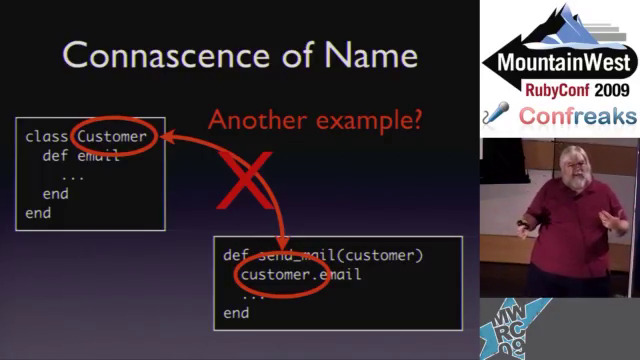
\includegraphics[height=.8\textheight]{weirich}}
  \end{center}
\end{frame}

\begin{frame}
  \frametitle{book by Meilir Page-Jones}
  \begin{center}
    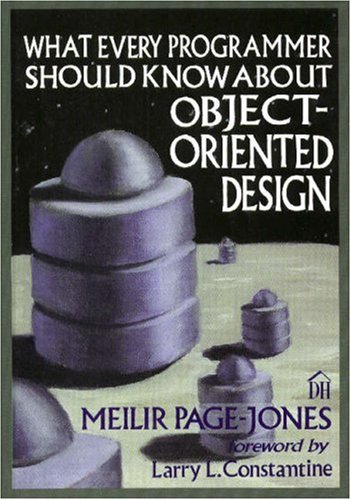
\includegraphics[height=.8\textheight]{meilir}
  \end{center}
\end{frame}

\begin{frame}
  \frametitle{connascence definition}
  Jim Weirich:\bigskip\\
  \begin{quote}
    Two pieces of software share \textbf{connascence} when a change in one requires a corresponding change in the other.
  \end{quote}
\end{frame}

\begin{frame}
  \frametitle{kinds of connascence ordered by increasing strength}
  \begin{center}
    \begin{tabular}{|l|l|l|}\hline
      & \textbf{abbreviation}  & \textbf{type} \\\hline
      \multirow{5}{*}{static}  & \textbf{CoN}  & Connascence of Name\\
      & \textbf{CoT}  & Connascence of Type\\
      & \textbf{CoM}  & Connascence of Meaning\\
      & \textbf{CoP}  & Connascence of Position\\
      & \textbf{CoA}  & Connascence of Algorithm\\\hline
      \multirow{4}{*}{dynamic} & \textbf{CoE}  & Connascence of Execution\\
      & \textbf{CoTi} & Connascence of Timing\\
      & \textbf{CoV}  & Connascence of Value\\
      & \textbf{CoI}  & Connascence of Identity\\\hline
    \end{tabular}\\\bigskip
    Also see \url{https://connascence.io/}
  \end{center}
\end{frame}

% examples for different kinds of connascence
% examples of code transformation to a kind of connascence with reduced strength
% strength, degree, and locality (modularity)

\end{document}
